\documentclass[10pt,a4paper]{article}

\usepackage{geometry}
\geometry{left=1cm, right=1cm, top=0.6cm, bottom=0.6cm}

\usepackage{fontspec}
\usepackage{xeCJK}
\usepackage{xcolor}
\usepackage{enumitem}
\usepackage{fontawesome5}
\usepackage{graphicx}
\usepackage{fancyhdr}
\usepackage[none]{hyphenat}

\setmainfont{Arial}
\setCJKmainfont[AutoFakeBold=true]{Microsoft YaHei}
\setCJKsansfont[AutoFakeBold=true]{Microsoft YaHei}
\setCJKmonofont[AutoFakeBold=true]{Microsoft YaHei}

% 调整行距与段落间距
\linespread{1.2} % 原图行距较紧凑，适当放大一点点防粘连
\setlength{\parskip}{0.2ex}


% 颜色定义
\definecolor{myblue}{RGB}{74,118,206}
\definecolor{tagblue}{RGB}{120,150,220}
\definecolor{tagbg}{RGB}{240,245,255} % 浅蓝色背景

\pagestyle{empty}

\newcommand{\cvsection}[2]{
  \vspace{0.6ex}
  \noindent{\color{myblue}\Large\bfseries\faIcon{#1}\hspace{0.5em}#2} \textcolor{myblue!50}{\hrulefill}\par
  \vspace{0.3ex}
}

% 定义小标签命令：带背景、圆角、垂直居中
\newcommand{\cvtag}[1]{%
  \raisebox{0.1ex}{%
    \setlength{\fboxsep}{1.5pt}%
    \colorbox{tagbg}{\textcolor{tagblue}{\fontsize{11pt}{13.2pt}\selectfont #1}}%
  }%
  \hspace{0.2em}%
}

% 自定义列表缩进与间距
\setlist[itemize,1]{leftmargin=0pt, label=, itemsep=0.4ex, topsep=0.4ex, parsep=0pt}
\setlist[itemize,2]{leftmargin=0.7em, label=$\circ$, itemsep=0.2ex, topsep=0.2ex, parsep=0pt}

\begin{document}

% 顶部个人信息区域
% 进一步利用 vspace 将整个头部向上提
\vspace*{-0.6cm}
% 取消左侧0.8\textwidth的限制，让名字部分占据全宽并强制居中
\begin{center}
  \textbf{\LARGE 马{\hspace{0.3em}}驰{\hspace{0.3em}}原}\\[0.5ex]
  13191869708 ~|~ machiyuan6@163.com ~|~ 2002-12 ~|~ 男 ~|~ 中共预备党员
\end{center}

% 照片绝对定位，从页面顶端对齐至教育经历横线
\begin{picture}(0,0)
  \put(440, 7){
    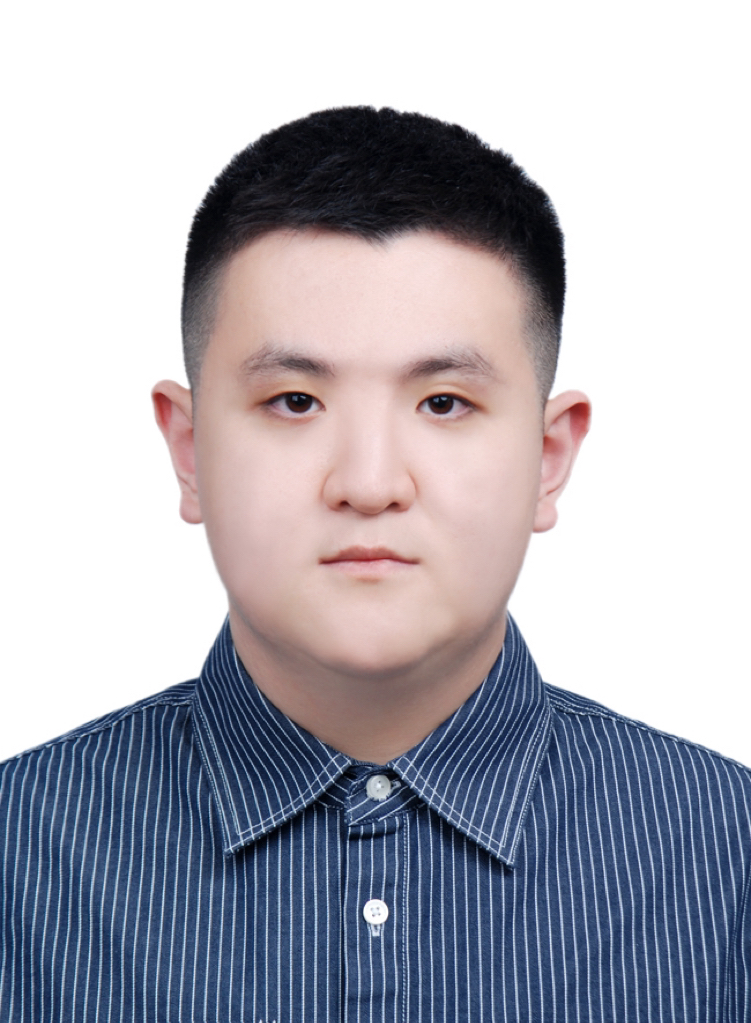
\includegraphics[height=2.4cm, keepaspectratio]{本科毕业证件照.jpg}
  }
\end{picture}
% 这里取消间距，把“教育经历”狠狠提上来
\vspace*{-1.2cm}

% 教育经历
\cvsection{graduation-cap}{教育经历}

{\fontsize{12pt}{14.4pt}\selectfont\noindent\textbf{东{\hspace{0.3em}}北{\hspace{0.3em}}大{\hspace{0.3em}}学} - 应用统计学 本科 \hspace{0.5em} \cvtag{985} \cvtag{211} \cvtag{双一流} \hfill 2021年09月 - 2025年07月\par}
\begin{itemize}[leftmargin=1em, label=, itemsep=0.35ex, topsep=0.05ex]
\item \textbf{【成绩\&课程】} \textbf{GPA: 3.7/4.0}；课程：Python，数学分析，概率论，运筹学；深度学习，仿真建模，时间序列等。
\item \textbf{【信息安全实验室】} 导师：\textbf{史闻博 教授}；协助研究生搭建区块链合约模拟系统，系统学习分布式架构、湖仓一体系统。
\end{itemize}
\vspace{0.3ex}

{\fontsize{12pt}{14.4pt}\selectfont\noindent\textbf{南洋理工大学} - 信号处理与机器学习 硕士 \hspace{0.5em} \cvtag{QS12} \cvtag{US28} \cvtag{软科88} \hfill 2025年08月 - 2026年08月\par}
\begin{itemize}[leftmargin=1em, label=, itemsep=0.35ex, topsep=0.05ex]
\item \textbf{【课程与科研】} \textbf{GPA: 3.9/5.0}；主修机器视觉、机器学习、视频信号处理等课程；\textbf{导师：Lin Zhiping 副教授、主任}。
\end{itemize}

% 实习经历
\cvsection{briefcase}{实习经历}

{\fontsize{12pt}{14.4pt}\selectfont\noindent\textbf{新加坡科技研究局 Astar} - I2R 资讯通信研究院 - 科研助理 \hfill 2025年09月 - 2026年07月\par}
\begin{itemize}[leftmargin=1em, label=, itemsep=0.35ex, topsep=0.05ex]
\item \textbf{【项目主导】} 主导开发 基于 \textbf{MHR} 的 面向治疗与运动训练的\textbf{人体动作精准指导AI系统}，独立完成项目动线设计；
\item \textbf{【架构设计】} 为解决定位,提出 \textbf{双轨空间解耦架构与交叉注意力机制},提取融合 2D姿态与 3D相机位姿,相机漂移\textbf{降低38\%};
\item \textbf{【运动学超分】} 为实现低代码运行，降低模型复杂度，研发基于 68 维 \textbf{One-hot} 的生成式 MLP 模型，将 17 个稀疏标记点上采样为全量骨骼的 6 自由度旋转数据，关键点误差\textbf{降低 50\% (至 0.6 mm)}，\textbf{CPU 推理速度达 >200 Hz}；
\item \textbf{【工程优化】} 多段参数由单独模型分别预测,实现体型与姿态特征解耦,同时集成 \textbf{自适应尺度估计}、\textbf{置信度加权 PnP} 及  \textbf{卡尔曼滤波}。系统在 \textbf{超2.7万帧} 多模态数据集上端到端平均误差仅 \textbf{4.2 mm},对齐延迟 \textbf{<5 ms},支持低算力 \textbf{>30 fps} 实时渲染
\end{itemize}
\vspace{0.3ex}

{\fontsize{12pt}{14.4pt}\selectfont\noindent\textbf{京{\hspace{0.3em}}东{\hspace{0.3em}}集{\hspace{0.3em}}团} - B端采销技术运营 - 汽车事业部 - 政企创新业务部 \hfill 2024年08月 - 2025年04月\par}
\begin{itemize}[leftmargin=1em, label=, itemsep=0.35ex, topsep=0.05ex]
\item {\fontsize{10.5pt}{12.6pt}\selectfont\textbf{【建模运营】}} \textbf{供应商入驻流程优化+经营分析打分模型，助力业务运营由纯人工把控过渡到客观模型量化}
  \begin{itemize}
    \item 经过业务调研，发现业务部门长期面临 \textit{B端入驻流程与标准C端流程不通用} 与 \textit{供应商量化监测缺失} 等问题；
    \item 针对 产能无法批量入驻 等问题,与PM重构流程并撰写全线指南文档,\textbf{OKR同比提高17\%},完结时效\textbf{由38h缩短至27h}；
    \item 使用 \textbf{Python} 构建针对供应商业绩的多因子权重模型，识别并淘汰僵尸商 \textbf{38家}，促进部门业绩季同比增加 \textbf{13\%}；
  \end{itemize}
\item {\fontsize{10.5pt}{12.6pt}\selectfont\textbf{【内部提效工具 0-1 孵化与迭代】}} \textbf{深入一线挖掘痛点，独立负责多款内部工具的规划、开发与落地，助力部门全流程提效。}
  \begin{itemize}
    \item 为减少采销沟通成本，利用 \textbf{Python} 制作名为"采销小助手"的微信外挂程序，并不断迭代；接入内部大模型言犀，保障合规性；设计\textbf{多层发送层}，结合\textbf{提示词工程}调整权重，隔离外部攻击风险；结合\textbf{流式传输}特点拼接响应，\textbf{首字延迟极低}；利用 \textbf{SR} 构建知识库，内存占用低且回复\textbf{准确率高}；使用前台模拟，累计回复\textbf{近十万条而未掉线}，\textbf{稳定性高}；
    \item 为方便部门发票管理，提升急标产出能力，独立完成发票信息抓取、打码及归档一体小程序的开发并迭代；囊括6种制式发票，总计处理\textbf{超 15000 份发票}，高峰期节省 \textbf{400 人力/天}，\textbf{提效 300\%}；打包为EXE程序，方便使用与传播；
    \item 为抓取大客户订单信息，制作爬虫遍历京东订单，\textbf{遵守机器人协议与合规要求}，抓取\textbf{共 3000 单}卡密，\textbf{近 30 万元}。
  \end{itemize}
\end{itemize}
\vspace{0.3ex}

{\fontsize{12pt}{14.4pt}\selectfont\noindent\textbf{河钢集团供应链管理有限公司} - 数据分析员 - 平台运营部 \hfill 2024年05月 - 2024年08月\par}
\begin{itemize}[leftmargin=1em, label=, itemsep=0.35ex, topsep=0.05ex]
\item \textbf{【评价建模】} 参与基于 \textbf{IAHP} 的钢厂风控模型评价指标制定、模型拟合等工作，为3个数据平台提供支持，\textbf{运行无失误}；
\item \textbf{【数据分析管理】} 利用 \textbf{SQL} 对子公司运费数据进行清洗和离群值分析，\textbf{抓取异常波动18次}；业务数据提取\textbf{共77次}，提取\textbf{效率}及\textbf{精细化处理}同期排名\textbf{小组第一}；参与业务工单分析，\textbf{词云分析}发现问题点\textbf{28项}，并与下游业务部门配合维护；
\item \textbf{【平台运营及拓展】} 参与 \textbf{Efree} 平台运营维护，解决合规异常点\textbf{超300项}；参与数字产品\textbf{数据资产认定}、入表、融资。
\end{itemize}

% 项目比赛经历
\cvsection{star}{项目比赛经历}

{\fontsize{12pt}{14.4pt}\selectfont\noindent\textbf{一种面向湖仓一体数据分析的隐私合规方法} - 本科组组长 \hfill 2022年03月 - 2023年12月\par}
\begin{itemize}[leftmargin=1em, label=, itemsep=0.35ex, topsep=0.05ex]
\item \textbf{【框架开发】} 为确保数据市场中数据分析的合规性与隐私性,设计以 \textbf{湖仓一体架构} 为基础的隐私合规框架,涉及法规遵从性验证层、TEE操作层、区块链存储层，物理层面保障数据隐私合规；创新引入声誉惩罚机制,\textbf{减少36\%}非授权的分析；
\item \textbf{【实验数据积累分析】} 共收集\textbf{300余条}运行时间量数据，倒推模型阻塞点\textbf{36处}，协助研究生完成验证，有效数据超\textbf{3G}；
\item \textbf{【项目成果1】} Ma, C., \& Hu, X. (2023). 湖仓一体化数据分析隐私合规方案. \textit{ACM ADMIT 2023, 10.1145/3625403.3625405}
\item \textbf{【项目成果2：发明专利授权】} 项目获得\textbf{中国发明专利授权}，验证了其创新性和实用性。
\end{itemize}
\vspace{0.3ex}

{\fontsize{12pt}{14.4pt}\selectfont\noindent\textbf{基于秦皇岛市民众对安宁疗护意愿的调查与问题研究} - 本科组组长 \hfill 2022年12月 - 2023年08月\par}
\begin{itemize}[leftmargin=1em, label=, itemsep=0.35ex, topsep=0.05ex]
\item \textbf{【问卷设计收集】} 调研"安宁疗护"产品受度；问卷精准投放，通过 \textbf{网络数据爬取} 和 \textbf{随机抽样} 等方法收集，共计\textbf{632份}；
\item \textbf{【实验建模】} 用 \textbf{描述性统计}、\textbf{Logistic模型}、\textbf{主成分分析}、\textbf{随机森林} 和 \textbf{K-means} 建立多权重模糊评价模型，\textbf{准确率 78\%}；
\item \textbf{【项目成果】} 第十三届全国大学生市场调查与分析大赛，\textbf{国家级三等奖}；第九届全国大学生统计建模大赛，\textbf{省级二等奖}。
\end{itemize}

% 个人总结
\cvsection{user}{个人总结}

\begin{itemize}[leftmargin=0pt, label=, itemsep=0.3ex, topsep=0.3ex]
\item \textbf{【荣誉】} 校三等奖学金5次；校创新创业奖学金2次(23\&24)；校优秀团干部/标兵(23\&24)；校三好学生(2023)等。
\item \textbf{【技能】} \textbf{Python>SQL>SPSS}；熟练使用 Antigravity 等\textbf{AI-Coding}工具，了解 Prompt 工程；\textbf{腾讯产品经理创造营进阶培训}。
\item \textbf{【自我评价】} 性格开朗；适应长期高压工作；善于组织、协调、沟通；有较强解决问题的能力与学习能力。
\end{itemize}

\end{document}
